\newpage

\section{Автоматическое определение релевантности параметров}
\subsection{Описание задачи}
Данная работа посвящена прореживанию структуры сети. Предлагается удалять наименее релевантные параметры модели. Под релевантностью~\cite{cun1990} подразумевается то, насколько параметр влияет на функцию ошибки. Малая релевантность указывает на то, что удаление этого параметра не влечет значимого изменения функции ошибки. Метод предлагает построение исходной избыточной сложности нейросети с большим количеством избыточных параметров. Для определения релевантности параметров предлагается оптимизацировать параметры и гиперпараметры в единой процедуре. Для удаления параметров предлагается использовать метод Белсли~\cite{neychev2016}.

\subsection{Постановка задачи}

Задана выборка
$$\mathfrak{D} = \{\textbf{x}_i,y_i\},~ i =1,...,N, \eqno(2.1)$$
где~$\textbf{x}_i \in \mathbb{R}^{m}$,~$y_i \in \{1, \dots, Y\}$,~$Y$ --- число классов.
Рассмотрим модель~$f(\mathbf{x}, \mathbf{w}): \mathbb{R}^m \times \mathbb{R}^n \to \{1,\dots,Y\}$, где~$\textbf{w} \in \mathbb{R}^n$ --- пространство параметров модели,

$$f(\mathbf{x}, \mathbf{w}) = \text{softmax}\bigl( f_1(f_2(...(f_l(\mathbf{x}, \mathbf{w})\bigr), \eqno(2.2)$$
где~$f_i(\mathbf{x}, \mathbf{w}) =  \text{tanh}(\mathbf{w}^\mathsf{T}\mathbf{x})$,~$l$ --- число слоев нейронной сети,~$i \in \{1\dots l\}$.
Параметр~$w_j$ модели~$f$  называется активным, если~$w_j \not = 0$. Множество индексов активных параметров обозначим~$\mathcal{A} \subset \mathcal{J} = \{1,...,n\}$.
Задано пространство параметров модели:
$$\mathbb{W_\mathcal{A}} = \{ \textbf{w} \in \mathbb{R}^n~|~w_j\not=0,~j \in \mathcal{A}  \}, \eqno(2.3)$$


Для модели~$f$ с множеством индексов активных параметров~$\mathcal{A}$ и соответствующего ей вектора параметров~$\textbf{w} \in \mathbb{W_\mathcal{A}}$  определим логарифмическую функцию правдоподобия выборки:
$$\mathcal{L}_\mathfrak{D}(\mathfrak{D}, \mathcal{A}, \textbf{w}) = \log p(\mathfrak{D}|\mathcal{A}, \textbf{w}), \eqno(2.4)$$
где~$p(\mathfrak{D}|\mathcal{A},\textbf{w})$ --- апостериорная вероятность выборки~$\mathfrak{D}$ при заданных~$\textbf{w}, \mathcal{A}$.
Оптимальные значения~$\textbf{w},\mathcal{A}$ находятся из минимизации~$-\mathcal{L}_{\mathcal{A}}(\mathfrak{D},\mathcal{A})$ --- логарифма правдоподобия модели:
$$\mathcal{L}_{\mathcal{A}}(\mathfrak{D},\mathcal{A}) =\log p(\mathfrak{D}|\mathcal{A}) = \log  \int_{{\textbf{w}\in\mathbb{W_\mathcal{J}}}}
p(\mathfrak{D} | \textbf{w}) p(\textbf{w} | \mathcal{A}) d \textbf{w}, \eqno(2.5)$$
где~$p(\textbf{w}|\mathcal{A})$ ---  априорная вероятность вектора параметров в пространстве~$\mathbb{W_\mathcal{J}}$.

Так как вычисление интеграла (2.5) является вычислительно сложной задачей, рассмотрим вариационный подход~\cite{bishop2006} для решения этой задачи. Пусть задано распределение~$q$:
$$q(\textbf{w})\sim \mathcal{N}(\textbf{m}, \textbf{A}^{-1}_\text{ps}), \eqno(2.6)$$
где~$\textbf{m}, \textbf{A}^{-1}_\text{ps}$ --- вектор средних и матрица ковариации, аппроксимирующее неизвестное апостериорное распределение~$p(\textbf{w}|\mathfrak{D},\mathcal{A})$:
$$p(\textbf{w} | \mathcal{A})\sim \mathcal{N}(\boldsymbol{\mu},\textbf{A}^{-1}_{\text{pr}}), \eqno(2.7)$$
где~$\boldsymbol{\mu},\textbf{A}^{-1}_{\text{pr}}$ --- вектор средних и матрица ковариации.

Приблизим интеграл (2.5) методом предложеном в \cite{bishop2006}:
$$\mathcal{L}_{\mathcal{A}}(\mathfrak{D},\mathcal{A}) = \log p(\mathfrak{D}|\mathcal{A}) = $$
$$ =\int_{\textbf{w}\in\mathbb{W_\mathcal{J}}} q(\textbf{w}) \log \frac{p(\mathfrak{D}, \textbf{w}|\mathcal{A})}{q(\textbf{w})}d \textbf{w} - \int_{\textbf{w}\in\mathbb{W_\mathcal{J}}}  q(\textbf{w}) \log \frac{p(\textbf{w}|\mathfrak{D},\mathcal{A})}{q(\textbf{w})}d \textbf{w} \approx $$
$$\approx \int_{\textbf{w}\in\mathbb{W_\mathcal{J}}} q(\textbf{w}) \log \frac{p(\mathfrak{D}, \textbf{w}|\mathcal{A})}{q(\textbf{w})}d \textbf{w} = $$
$$= \int_{\textbf{w}\in\mathbb{W_\mathcal{J}}} q(\textbf{w}) \log \frac{p(\textbf{w}| \mathcal{A})}{q(\textbf{w})}d \textbf{w} + \int_{\textbf{w}\in\mathbb{W_\mathcal{J}}} q(\textbf{w}) \log p(\mathfrak{D}|\mathcal{A}, \textbf{w})d \textbf{w}=$$

$$=\mathcal{L}_\textbf{w}(\mathfrak{D}, \mathcal{A}, \textbf{w})+\mathcal{L}_{E}(\mathfrak{D},\mathcal{A}). \eqno(2.8)$$

Первое слагаемое формулы (2.8) --- это сложность модели. Оно определяется расстоянием Кульбака-Лейблера:
$$\mathcal{L}_\textbf{w}(\mathfrak{D}, \mathcal{A}, \textbf{w}) = -D_{KL}\bigl(q(\textbf{w})||p(\textbf{w}|\mathcal{A})\bigr). \eqno(2.9)$$
Второе слагаемое формулы (2.8) является матожиданием правдоподобия выборки~$\mathcal{L}_\mathfrak{D}(\mathfrak{D},\mathcal{A}, \textbf{w})$. В данной работе оно является функцией ошибки:
$$\mathcal{L}_{E}(\mathfrak{D},\mathcal{A}) = \mathsf{E}_{\textbf{w}\sim q}\mathcal{L}_\mathfrak{D}(\textbf{y}, \mathfrak{D}, \mathcal{A}, \textbf{w}). \eqno(2.10)$$

Требуется найти параметры, доcтавляющие минимум суммарному функционалу потерь~$\mathcal{L}_\mathcal{A}(\mathfrak{D},\mathcal{A},\textbf{w})$ из (2.8):
$$\hat{\textbf{w}} = \argmin_{\mathcal{A}\subset\mathcal{J},~\textbf{w} \in \mathbb{W_\mathcal{A}}} -\mathcal{L}_\mathcal{A}(\mathfrak{D}, \mathcal{A}, \textbf{w}) = $$
$$=\argmin_{\mathcal{A}\subset\mathcal{J},~\textbf{w} \in \mathbb{W_\mathcal{A}}} D_{KL}\bigl(q(\textbf{w})||p(\textbf{w}|\mathcal{A})\bigr) - \mathcal{L}_\mathfrak{D}(\mathfrak{D}, \mathcal{A}, \textbf{w}). \eqno(2.11)$$

\subsection{Случайное удаление}
Метод случайного удаления заключается в том, что случайным образом удаляется некоторый параметр $w_\xi$ из множества активных параметров сети.  Индекс параметра $\xi$ из равномерного распределения  случайная величина, предположительно доставляющая оптимум в (2.11).
$$\xi \sim \mathcal{U}(\mathcal{A}). \eqno(3.1.1)$$

\subsection{Оптимальное прореживание}
Метод оптимального прореживания \cite{cun1990} использует вторую производную целевой функции (2.4) по параметрам для определения нерелевантных параметров. Рассмотрим функцию потерь~$\mathcal{L}$ (2.4) разложенную в ряд Тейлора в некоторой окрестности вектора параметров~$\textbf{w}$:
$$\delta \mathcal{L} = \sum_{j\in \mathcal{A}} g_j\delta w_j + \frac{1}{2}\sum_{i,j\in \mathcal{A}} h_{ij}\delta w_i\delta w_j + O(||\delta\textbf{w}||^3), \eqno(3.2.1)$$
где~$\delta w_j~$ --- компоненты вектора~$\delta\textbf{w}$,~$g_j$ --- компоненты вектора градиента~$\nabla \mathcal{L}$, а~$h_{ij}$ --- компоненты гесcиана~$\textbf{H}$:
$$g_j = \frac{\partial \mathcal{L}}{\partial w_j}, \qquad h_{ij} = \frac{\partial^2\mathcal{L}}{\partial w_i \partial w_j}. \eqno(3.2.2)$$

Задача является вычислительно сложной в силу размерности матрицы \textbf{H}. Введем следующее предположение \cite{cun1990}, о том что удаление нескольких параметров приводит к такому же изменению функции потерь~$\mathcal{L}$, как и суммарное изменение при индивидуальном удалении:
$$\delta \mathcal{L} = \sum_{j\in \mathcal{A}} \delta \mathcal{L}_j, \eqno(3.2.3)$$
где~$\mathcal{A}$ --- множество активных параметров,~$\delta\mathcal{L}_j$ --- изменение функции потерь, при удалении одного параметра~$\textbf{w}_j$.

В силу данного предположения будем рассматривать только диагональные элементы матрицы \textbf{H}. После введенного предположения, выражение (3.2.1) принимает вид
$$\delta \mathcal{L} = \frac{1}{2} \sum_{j\in \mathcal{A}} h_{jj}\delta w_j^2, \eqno(3.2.4)$$

Получаем следующую задачу оптимизации:

$$\xi = \argmin_{j\in \mathcal{A}} h_{jj}\frac{w_j^2}{2}, \eqno(3.2.5)$$
где~$\xi$ --- индекс наименее релевантного, удаляемого параметра, предположительно доставляющая оптимум в (2.11).

\subsection{Удаление неинформативных параметров с помощью вариационного вывода}
Для удаления параметров в работе \cite{graves2011} предлагается удалить параметры, которые имеют максимальное отношение плотности~$p(\textbf{w}|\mathcal{A})$ априорной вероятности в нуле к плотности вероятности априорной вероятности в математическом ожидании параметра.\\
Для гауссовского распределения с диагональной матрицей ковариации получаем:
$$p_j(\textbf{w}|\mathcal{A})(x) = \frac{1}{\sqrt[]{2\sigma_j^2}}\exp({-\frac{(x-\mu_j)^2}{2\sigma_j^2}}). \eqno(3.3.1)$$
Разделив плотность вероятности в нуле к плотности в математическом ожидание
$$ \frac{p_j(\textbf{w}|\mathcal{A})(0)}{p_j(\textbf{w}|\mathcal{A})(\mu_j)}= \exp({-\frac{\mu_j^2}{2\sigma_j^2}}), \eqno(3.3.2)$$
Получаем следующую задачу оптимизации:
$$\xi = \argmin_{j\in \mathcal{A}} \left|\frac{\mu_j}{\sigma_j}\right|, \eqno(3.3.3)$$
где~$\xi$ --- индекс наименее релевантного, удаляемого параметра.

\subsection{Прореживание сети на основе метода Белсли}
Предлагается метод основанный на модификации метода Белсли. Пусть $\textbf{w}$ --- вектор параметров доставляющий минимум функционалу потерь $\mathcal{L}$ на  множестве $\mathbb{W_\mathcal{A}}$, а $\textbf{A}_\text{ps}$ соответствующая ему ковариационная матрица.

Выполним сингулярное разложение матрицы
$$\textbf{A}_\text{ps} = \textbf{U}{\bf\Lambda}\textbf{V}^\mathsf{T}. \eqno(4.1)$$
Индекс обусловленности $\eta_{j}$ определим как отношение максимального элемента к $j$-му элементу матрицы ${\bf\Lambda}$. Для нахождения мультиколлиниарных признаков требуется найти индекс~$\xi$ вида:
$$\xi = \argmax_{j\in \mathcal{A}}{\eta_j}. \eqno(4.2)$$

\begin{figure}[h!t]\center
\subfloat[Матрица ковариации]{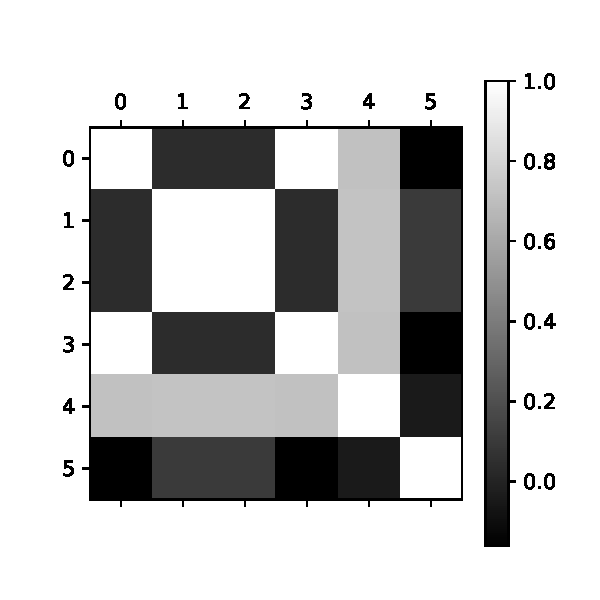
\includegraphics[width=0.5\textwidth]{results/relevant/Cov.pdf}}
\subfloat[Дисперсионные доли]{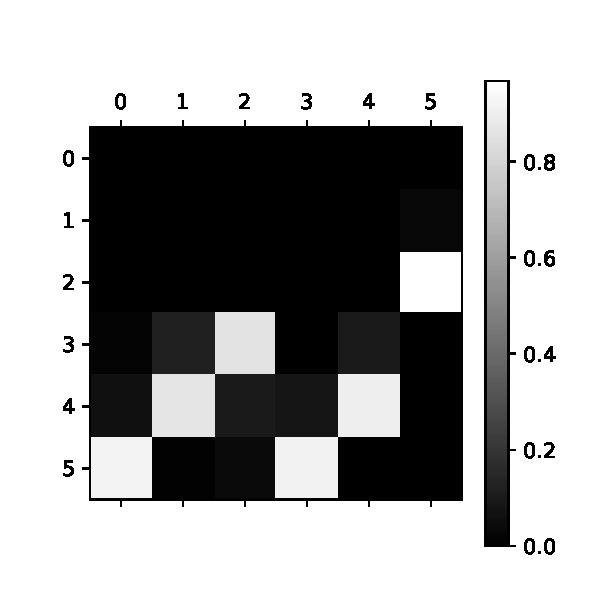
\includegraphics[width=0.5\textwidth]{results/relevant/BelslyImage.pdf}}
\caption{Илюстрация метода Белсли}
\label{CovBel}
\end{figure}

\begin{table}[h]
\begin{center}
\caption{Илюстрация метода Белсли}
\begin{tabular}{|c|cccccc|}
\hline
$\eta$ & $q_1$& $q_2$& $q_3$& $q_4$& $q_5$& $q_6$\\
\hline
$1.0$ &  $2\cdot 10^{-17}$ &  $4\cdot 10^{-17}$ &  $1\cdot 10^{-16}$ &  $2\cdot 10^{-17}$ &  $6\cdot 10^{-17}$&  $3\cdot 10^{-4}$ \\
\hline
$1.5$ &  $5\cdot 10^{-17}$ &  $9\cdot 10^{-17}$ &  $2\cdot 10^{-16}$ &  $5\cdot 10^{-17}$ &  $3\cdot 10^{-20}$ &  $3\cdot 10^{-2}$ \\
\hline
$3.3$ &  $9\cdot 10^{-18}$ &  $1\cdot 10^{-17}$ &  $2\cdot 10^{-17}$ &  $9\cdot 10^{-18}$ &  $2\cdot 10^{-19}$ &  $9\cdot 10^{-1}$ \\
\hline
$2\cdot 10^{15}$ &  $1\cdot 10^{-2}$ &  $1\cdot 10^{-1}$ &  $8\cdot 10^{-1}$ &  $2\cdot 10^{-3}$ &  $9\cdot 10^{-2}$ &  $1\cdot 10^{17}$ \\ 
\hline
$8\cdot 10^{15}$ &  $6\cdot 10^{-2}$ &  $8\cdot 10^{-1}$ &  $9\cdot 10^{-2}$ &  $8\cdot 10^{-2}$ &  $9\cdot 10^{-1}$ & $ 2\cdot 10^{17} $\\
\hline
$1\cdot 10^{16}$ &  $\bf9\cdot 10^{-1}$ &  $1\cdot 10^{-2}$& $ 4\cdot 10^{-2}$&  $\bf9\cdot 10^{-1}$ &  $1\cdot 10^{-3}$ & $ 5\cdot 10^{-21}$ \\
\hline
\end{tabular}
\label{CovBelTable}
\end{center}
\end{table}

Дисперсионный долевой коэффициент $q_{ij}$ определим как вклад $j$-го признака в дисперсию $i$-го элемента вектора параметра~$\textbf{w}$:

$$q_{ij} = \frac{u^2_{ij}/\lambda_{jj}}{\sum^n_{j=1}{u^2_{ij}/\lambda_{jj}}}. \eqno(4.3)$$

Большие значение дисперсионных долей указывают на наличие зависимости между параметрами. Находим долевые коэффициенты, которые вносят максимальный вклад в дисперсию параметра~$w_\xi$:

$$\zeta = \argmax_{j\in \mathcal{A}}{q_{\xi j}}. \eqno(4.4)$$
Параметр с индексом $\zeta$ определим как наименее релевантный параметр нейросети. 
%Для удаления нескольких зависимых параметров за раз, предлагается удалить параметры с номерами $p \in \mathcal{A}: q_{\xi i} > \lambda  \in  \mathbb{R}_+$.

Проиллюстрируем принцип работы метода Белсли на примере. Рассмотрим данные порожденные следующим образом: 
$$\textbf{w} = \begin{bmatrix}
\text{sin}(x)\\
\text{cos}(x)\\
\text{2+cos}(x)\\
\text{2+sin}(x)\\
\text{cos}(x) + \text{sin}(x)\\
x
\end{bmatrix}$$
с матрицей ковариации на рис.~\ref{CovBel}.a, где $x \in [0.0, 0.02, ..., 20.0]$.


В табл.~\ref{CovBelTable} приведены индексы обусловленности и соответствующие им дисперсионные доли, которые также изображены на рис.~\ref{CovBel}.b. Согласно этим данным, максимальный индекс обусловленности $\eta_6 = 1.2\cdot 10^{16}$. Ему соответствуют максимальные дисперсионные доли признаков с индексами 1 и 4, которые, как видно из построения выборки, являются линейно зависимые.

\subsection{Вычислительный эксперимент}
Для анализа свойств предложенного алгоритма и сравнения его с существующими был проведен вычислительный эксперимент в котором параметры нейросети удалялись методами,  которые были описаны в разделах 3.1---3.3 и методом Белсли.

В качестве данных использовались три выборки. Выборки Wine~\cite{Wine} и Boston~Housing~\cite{Boston}  --- это реальные данные. Синтетические данные сгенерированы таким образом чтобы параметры сети были мультиколинеарными. Генерация данных состояла из двух этапов. 
На первом этапе генерировался вектор параметров $\mathbf{w}_{\text{synthetic}}$:
$$\mathbf{w}_{\text{synthetic}}  \sim \mathcal{N}(\textbf{m}_{\text{synthetic}}, \textbf{A}_{\text{synthetic}}), \eqno(5.1)$$ 
где 
$\textbf{m}_{\text{synthetic}} = \begin{bmatrix}
1.0\\
0.0025\\
\cdots\\
0.0025
\end{bmatrix}$,
$\textbf{A}_{\text{synthetic}} = \begin{bmatrix}
1.0& 10^{-3}& \cdots& 10^{-3}& 10^{-3}\\
10^{-3}& 1.0& \cdots& 0.95& 0.95\\
\cdots&\cdots&\cdots&\cdots&\cdots\\
10^{-3}& 0.95& \cdots& 0.95& 1.0
\end{bmatrix}$.

На втором этапе генерировалась выборка $\mathfrak{D}_{\text{synthetic}}$:
$$\mathfrak{D}_{\text{synthetic}} = \{(\textbf{x}_i,y_i)| \textbf{x}_i \sim  \mathcal{N}(\textbf{1}, \textbf{I}), y_i = x_{i0}, i = 1 \cdots 10000\}. \eqno(5.2)$$
В приведенном выше векторе параметров $\mathbf{w}_{\text{synthetic}}$ для выборки $\mathfrak{D}_{\text{synthetic}}$, наиболее релевантным является первый параметр, а все остальные параметры являются нерелевантными. Матрица ковариации была выбрана таким образом, чтобы все нерелевантные параметры были зависимы и метод Белсли был максимально эффективен.



\begin{table}[h]

\begin{center}
\caption{Описание выборок}
\begin{tabular}{|c|c|c|c|}
\hline
	Выборка &Тип задачи& Размер выборки& Число признаков\\
	\hline
	
	\multicolumn{1}{|l|}{Wine}
	&
	\multicolumn{1}{|l|}{класификация}
	 & 178 & 13\\
	\hline
	
	\multicolumn{1}{|l|}{Boston Housing}
	&
	\multicolumn{1}{|l|}{регресия}
	& 506 & 13\\
	\hline
	
	\multicolumn{1}{|l|}{Synthetic data}
	&
	\multicolumn{1}{|l|}{регресия}
	& 10000 & 100\\
\hline

\end{tabular}
\end{center}
\end{table}



Для алгоритмов тренировочная и тестовая выборки составили~$80\%$ и~$20\%$ соответсвенно. Критерием качества прореживания служит процент параметров нейросети, удаление которого не влечет значимой потери качества прогноза. Также критерием качества служит устойчивость нейросети к зашумленности данных. 

Качеством прогноза $R_{\text{cl}}$ модели для задачи классификации является точность прогноза модели:
$$R_{\text{cl}} = \frac{\sum_{(\textbf{x},y)\in \mathfrak{D}} [f(\textbf{x}, \textbf{w}) = y]}{\left|\mathfrak{D}\right|}, \eqno(5.3)$$

Качеством прогноза $R_{\text{rg}} $ модели для задачи регрессии является среднеквадратическое отклонение результата модели от точного:

$$R_{\text{rg}} = \frac{\sum_{(\textbf{x},y)\in \mathfrak{D}} \left(f(\textbf{x}, \textbf{w}) - y\right)^2}{\left|\mathfrak{D}\right|}, \eqno(5.4)$$

\paragraph{Wine.} Рассмотрим нейроную сеть с 13 нейронами на входе, 13 нейронами в скрытом слое и 3 нейронами на выходе.

\begin{figure}[h!t]\center
\includegraphics[width=0.8\textwidth]{results/relevant/WIne/All.pdf}\\
\caption{Качество прогноза при удаление параметров на выборке Wine}
\label{WineAll}
\end{figure}

\begin{figure}[h!t]\center
\subfloat[Произвольное удаление параметров]{\includegraphics[width=0.5\textwidth]{results/relevant/WIne/RandomNoise3D.pdf}}
\subfloat[Оптимальное прореживание]{\includegraphics[width=0.5\textwidth]{results/relevant/WIne/OBDNoise3D.pdf}}\\
\subfloat[Вариационный метод]{\includegraphics[width=0.5\textwidth]{results/relevant/WIne/VariationalNoise3D.pdf}}
\caption{Влияние шума в начальных данных на шум выхода нейросети на выборке Wine}
\label{WineNoise}
\end{figure}

На рис.~\ref{WineAll} показано как меняется точность прогноза $R_{\text{cl}}$ при удалении параметров указанными методами. Из графика видно, что метод оптимального прореживания, вариационный метод и метод Белсли позволяют удалить $\approx80\%$ параметров и качество всех этих методов падает при удалении $\approx90\%$ параметров нейросети. 

На рис.~\ref{WineNoise} показаны поверхности изменения уровня шума ответов нейросети при изменении процента удаленных параметров и уровня шума входных данных для разных методов прореживания. На графиках показано, что при удалении параметров нейросети методом Белсли шум меньше, чем при удалении параметров другими методами, на это указывает то что поверхность которая соответствует методу Белсли ниже других поверхностей.

\paragraph{Boston Housing.} Рассмотрим нейроную сеть с 13 нейронами на входе, 39 нейронами в скрытом слое и одним нейроном на выходе.

\begin{figure}[h!t]\center
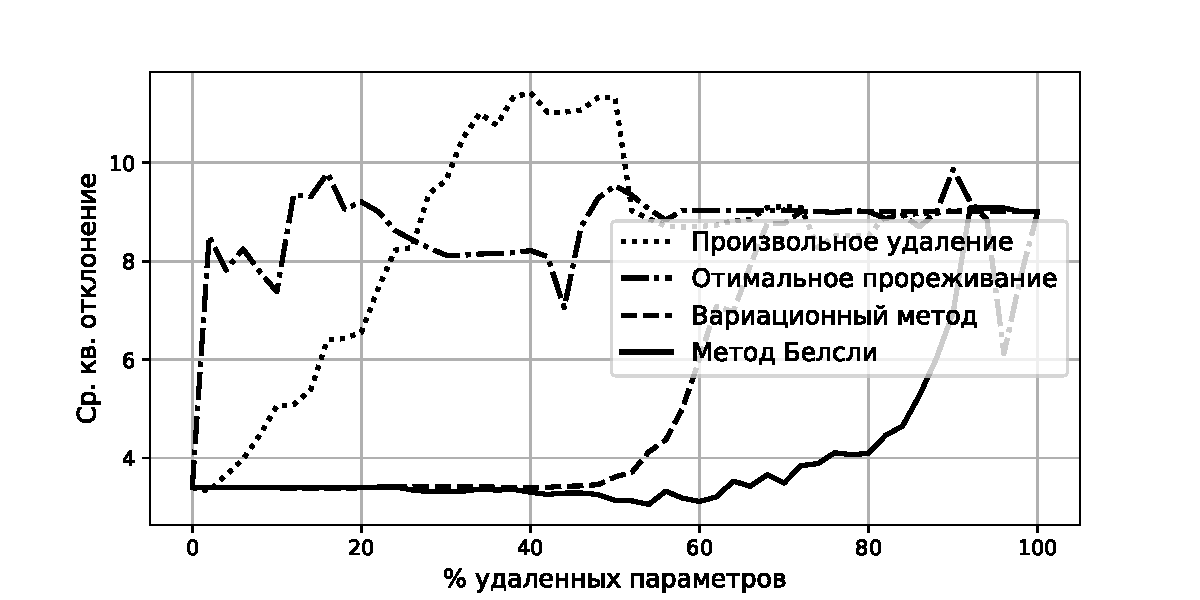
\includegraphics[width=0.8\textwidth]{results/relevant/Boston/All.pdf}\\
\caption{Качество прогноза при удаление параметров на выборке Boston}
\label{BostonAll}
\end{figure}

\begin{figure}[h!t]\center
\subfloat[Произвольное удаление параметров]{\includegraphics[width=0.5\textwidth]{results/relevant/Boston/RandomNoise3D.pdf}}
\subfloat[Оптимальное прореживание]{\includegraphics[width=0.5\textwidth]{results/relevant/Boston/OBDNoise3D.pdf}}\\
\subfloat[Вариационный метод]{\includegraphics[width=0.5\textwidth]{results/relevant/Boston/VariationalNoise3D.pdf}}
\caption{Влияние шума в начальных данных на шум выхода нейросети на выборке Boston}
\label{BostonNoise}
\end{figure}

На рис.~\ref{BostonAll} показано как меняется среднеквадратическое отклонение прогноза $\mathsf{R}_{\text{rg}}$ от точного ответа  при удалении параметров указанными методами. График показывает, что метод Белсли является более эффективным, чем другие методы, так-как позволяет удалить больше параметров нейросети без потери качества.

На рис.~\ref{BostonNoise} показаны поверхности изменения уровня шума ответов нейросети при изменении процента удаленных параметров и уровня шума входных данных для разных методов прореживания. График показывает, что уровень шума всех методов одинаковый, так-как поверхности всех методов находятся на одном уровне.


\paragraph{Синтетические данные.} Рассмотрим нейроную сеть с 100 нейронами на входе и одним нейроном на выходе.

\begin{figure}[h!t]\center
\includegraphics[width=0.8\textwidth]{results/relevant/Data1/All.pdf}\\
\caption{Качество прогноза при удаление параметров на синтетической выборке}
\label{Data1All}
\end{figure}

\begin{figure}[h!t]\center
\subfloat[Произвольное удаление параметров]{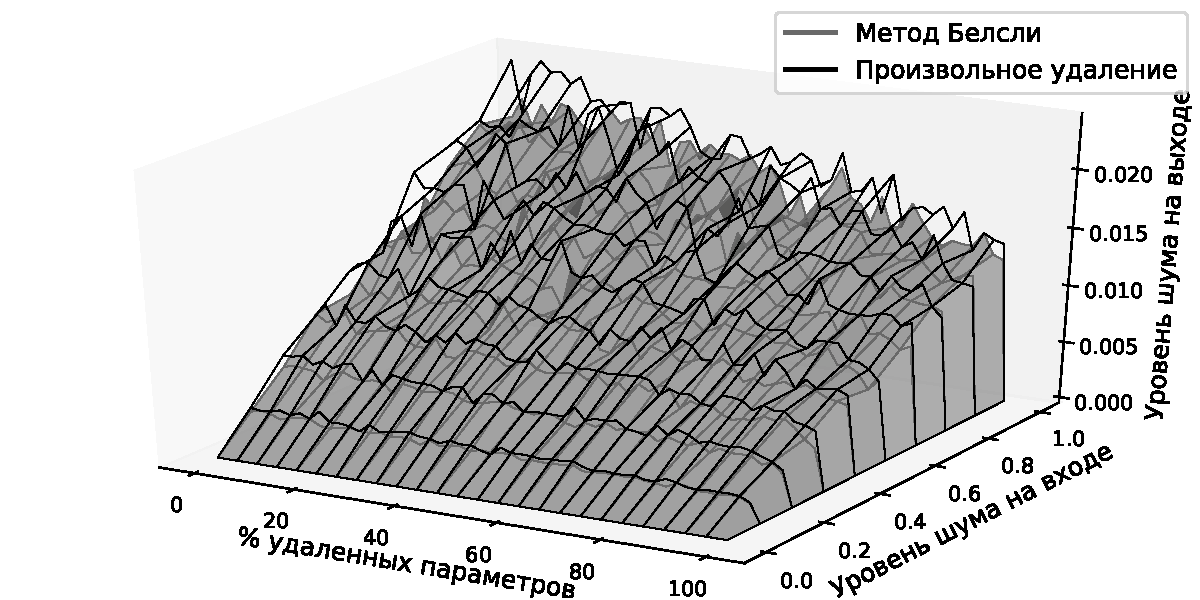
\includegraphics[width=0.5\textwidth]{results/relevant/Data1/RandomNoise3D.pdf}}
\subfloat[Оптимальное прореживание]{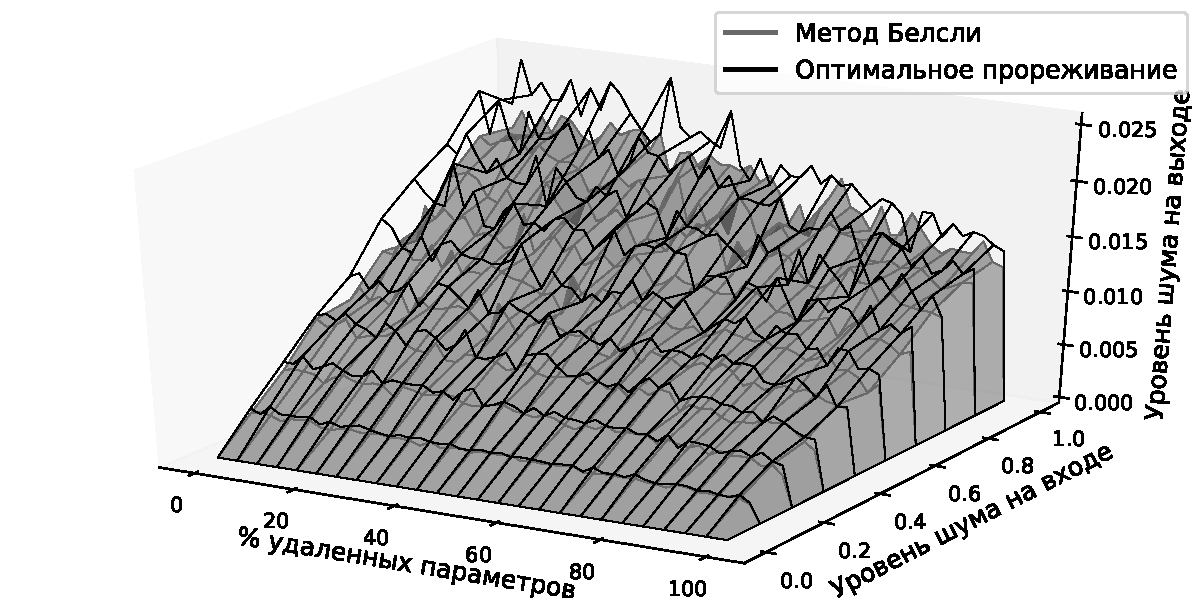
\includegraphics[width=0.5\textwidth]{results/relevant/Data1/OBDNoise3D.pdf}}\\
\subfloat[Вариационный метод]{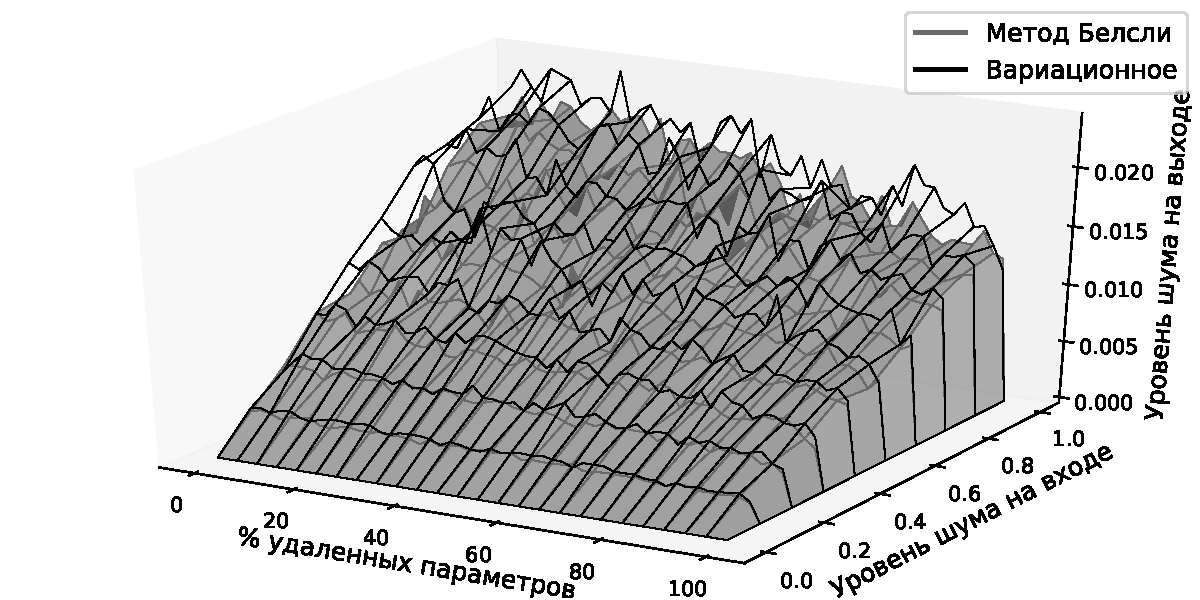
\includegraphics[width=0.5\textwidth]{results/relevant/Data1/VariationalNoise3D.pdf}}
\caption{Влияние шума в начальных данных на шум выхода нейросети на синтетической выборке}
\label{Data1Noise}
\end{figure}

На рис.~\ref{Data1All} показано как меняется среднеквадратическое отклонение прогноза от $\mathsf{R}_{\text{rg}}$ точного ответа при удалении параметров указанными методами. График показывает, что удаление параметров методом Белсли являеться более эффективным чем другие методы прореживания, так-как качество прогноза нейросети улучшается при удалении шумовых параметров.

На рис.~\ref{Data1Noise} показаны поверхности изменения уровня шума ответов нейросети при изменении процента удаленных параметров и уровня шума входных данных для разных методов прореживания. На графиках показано, что при удалении параметров нейросети методом Белсли шум меньше, чем при удалении параметров другими методами, так-как поверхность которая соответствует методу Белсли ниже других поверхностей.
